%! Unidad 9 — Cinemática aplicada: movimientos rectilíneos, composición de movimientos y movimiento circular
%! (teoría, ejemplos resueltos, ejercicios por apartados, lectura, prácticas y situación de aprendizaje)
%! Fuente: Fuentes/Fisica/Unidad 9 (capturas 202-216, solucionario) y Unidad 10 (captura 217: olimpiadas y autoevaluación).
%! Texto reescrito; datos de los ejercicios cambiados y recalculados. Se usa g = 9,8 m/s² en todo el tema.
%! Figuras en images/UD9/: nuevas en html/ (composicion_rio, tiro_parabolico, tiro_horizontal, mesa_rampa), adaptadas de
%!   4ESO/images/UD9/html (mcu_magnitudes, mcu_vectores: θ cambiado por φ; usan fig_circular.js) y copiadas (PDF + SVG)
%!   de 4ESO/images/UD7 (lanzamiento_vertical, plano_galileo). Gráficas x-t, v-t y a-t con pgfplots (estilo «grafica»).

\section*{Para empezar: saltos de \textit{freestyle}}
\addcontentsline{toc}{section}{Para empezar: saltos de \textit{freestyle}}

En una competición de \textit{freestyle} de motocross, los pilotos aceleran por una recta, toman curvas, suben por una rampa y salen
volando varios metros por encima del suelo mientras hacen acrobacias. Durante el salto, la moto describe una \textbf{parábola}: su
movimiento es la combinación de un avance horizontal a velocidad constante y una subida y bajada como la de una pelota lanzada hacia
arriba. Mientras tanto, las ruedas siguen girando con un \textbf{movimiento circular}.

En la unidad anterior aprendimos a describir cualquier movimiento con vectores. Ahora aplicaremos esas herramientas a los movimientos
más importantes: los \textbf{rectilíneos} (uniforme y uniformemente acelerado, incluida la caída libre), los \textbf{compuestos}
(cruzar un río, lanzar un balón a canasta) y los \textbf{circulares}.

%========================================================================================
\section{Recuerda de la ESO}\label{sec:ud9-eso}
%========================================================================================

\paragraph{Clasificación de los movimientos.} Según las componentes intrínsecas de la aceleración, los movimientos pueden ser:

\begin{table}[H]
    \centering
    \caption{Clasificación de los movimientos según su aceleración}
    \vspace{-5pt}
    \begin{tabular}{@{}llL{5.6cm}@{}}
        \toprule
        \textbf{Trayectoria} & \textbf{Movimiento} & \textbf{Características} \\
        \midrule
        \multirow{2}{*}{Rectilínea (\(a_n = 0\))} & Uniforme (MRU) & \(v\) constante; \(a_t = 0\). Ej.: un tren en un tramo recto a velocidad constante \\[3pt]
         & Uniformemente acelerado (MRUA) & \(a_t\) constante. Ej.: una piedra que cae \\[3pt]
        \multirow{2}{*}{Circular (\(a_n \neq 0\))} & Uniforme (MCU) & Rapidez constante; \(a_t = 0\). Ej.: la rueda de una jaula de hámster \\[3pt]
         & Uniformemente acelerado (MCUA) & Aceleración angular constante. Ej.: las aspas de un ventilador al encenderlo \\
        \bottomrule
    \end{tabular}
    \label{tab:ud9-clasificacion}
\end{table}

\paragraph{El radián.} Es la unidad de ángulo del SI: un \textbf{radián} es el ángulo cuyo arco mide lo mismo que el radio. Como la
circunferencia mide \(2\pi R\), una vuelta completa son \(2\pi\)~rad, es decir, \(360^\circ = 2\pi\)~rad y
\(180^\circ = \pi\)~rad. Para pasar de revoluciones por minuto (rpm) a rad/s:
\[ 3000~\frac{\text{vueltas}}{\unit{\minute}} \cdot \frac{2\pi~\text{rad}}{1~\text{vuelta}} \cdot \frac{\qty{1}{\minute}}{\qty{60}{\s}} = 100\pi~\unit{\radian\per\s} \]

\paragraph{Representaciones gráficas.} En cinemática se representa el tiempo en el eje horizontal y la posición, la velocidad o la
aceleración en el vertical. Una función de primer grado, \(y = mx + n\), es una \textbf{recta} de pendiente \(m\); una de segundo
grado, \(y = ax^2 + bx + c\), es una \textbf{parábola}, cóncava hacia arriba si \(a > 0\) y hacia abajo si \(a < 0\), con el vértice
en \(x_v = -\dfrac{b}{2a}\).

\begin{exercise}
    a) Expresa \(150^\circ\) en radianes y \qty{2.5}{\radian} en grados. b) Expresa \qty{1200}{rpm} en \unit{\radian\per\s} y
    \qty{3}{\radian\per\s} en rpm.
    \begin{solu}
        a) \(150 \cdot \dfrac{\pi}{180} = \dfrac{5\pi}{6} = \textcolor{red}{\qty{2.62}{\radian}}\); \(\num{2.5} \cdot \dfrac{180}{\pi} =
        \textcolor{red}{143{,}2^\circ}\). b) \(1200 \cdot \dfrac{2\pi}{60} = 40\pi = \textcolor{red}{\qty{125.7}{\radian\per\s}}\);
        \(3 \cdot \dfrac{60}{2\pi} = \textcolor{red}{\qty{28.6}{rpm}}\).
    \end{solu}
\end{exercise}

\begin{exercise}
    Representa las funciones \(y = 2x - 1\) e \(y = x^2 - 4x + 3\). Indica la pendiente de la primera y el vértice y los cortes
    con el eje X de la segunda.
    \begin{solu}
        \textcolor{red}{Recta de pendiente 2} que corta al eje Y en \(-1\). \textcolor{red}{Parábola cóncava hacia arriba}, con vértice
        en \(x_v = 2\), \(\textcolor{red}{(2, -1)}\), que corta al eje X en \(\textcolor{red}{x = 1}\) y \(\textcolor{red}{x = 3}\).
    \end{solu}
\end{exercise}

%========================================================================================
\section{El movimiento rectilíneo}\label{sec:ud9-rectilineo}
%========================================================================================

En un \textbf{movimiento rectilíneo} la trayectoria es una recta y la velocidad no cambia de dirección, así que \(a_n = 0\). Lo más
cómodo es colocar un eje (X si el movimiento es horizontal, Y si es vertical) sobre la propia trayectoria: los vectores se reducen
entonces a números con signo. Distinguiremos dos casos, según que la velocidad cambie de módulo (\(a_t \neq 0\)) o no (\(a_t = 0\)).

\subsection{Movimiento rectilíneo uniforme (MRU)}

\begin{definition}[MRU]
    En el \textbf{movimiento rectilíneo uniforme} la trayectoria es una recta y el vector velocidad es \textbf{constante} en módulo,
    dirección y sentido: \(\vec a = \vec 0\). El móvil recorre \textbf{distancias iguales en tiempos iguales}.
\end{definition}

\subsubsection{Ecuación del movimiento}

Como no hay aceleración, la velocidad media y la instantánea coinciden siempre:
\[ \vec v = \vec v_m = \frac{\vec r - \vec r_0}{t - t_0} \quad\Rightarrow\quad \vec r = \vec r_0 + \vec v\,(t - t_0) \]
Si tomamos el eje X sobre la trayectoria y empezamos a contar el tiempo en \(t_0 = 0\):
\[ \boxed{x = x_0 + v\,t} \qquad\qquad (\text{o } y = y_0 + v\,t \text{ en un movimiento vertical}) \]
donde \(x_0\) es la posición inicial. El \textbf{signo} de \(v\) indica el sentido: positivo hacia la derecha (o hacia arriba) y
negativo hacia la izquierda (o hacia abajo). Cuidado: si hay varios móviles que no empiezan a moverse a la vez, el tiempo que lleva
moviéndose cada uno es \(t - t_0\), no \(t\).

\subsubsection{Gráficas del MRU}

\begin{figure}[H]
    \centering
    \begin{tikzpicture}
        \begin{axis}[grafica, width=0.36\linewidth, xlabel={\(t\)}, ylabel={\(x\)}, xmin=0, xmax=6, ymin=0, ymax=10, xtick=\empty, ytick={2}, yticklabels={\(x_0\)}]
            \addplot[very thick, ocre, domain=0:6] {2 + 1.2*x} node[pos=0.8, above left, font=\scriptsize] {\(v > 0\)};
            \addplot[very thick, blue!70!black, domain=0:6] {9 - 1.2*x} node[pos=0.6, above right, font=\scriptsize] {\(v < 0\)};
        \end{axis}
    \end{tikzpicture}\hspace{1cm}
    \begin{tikzpicture}
        \begin{axis}[grafica, width=0.36\linewidth, xlabel={\(t\)}, ylabel={\(v\)}, xmin=0, xmax=6, ymin=0, ymax=4, xtick={1,4}, xticklabels={\(t_1\),\(t_2\)}, ytick={3}, yticklabels={\(v\)}]
            \addplot[fill=ocre!25, draw=none, domain=1:4] {3} \closedcycle;
            \addplot[very thick, ocre, domain=0:6] {3};
            \node[font=\scriptsize] at (axis cs:2.5,1.5) {\(\Delta x = v\,\Delta t\)};
        \end{axis}
    \end{tikzpicture}
    \caption{Gráficas del MRU. Posición-tiempo: una recta cuya pendiente es la velocidad. Velocidad-tiempo: una recta horizontal;
    el área bajo ella es el desplazamiento.}
    \label{fig:ud9-graficas-mru}
\end{figure}

\begin{itemize}
    \item La gráfica \(x\)-\(t\) es una \textbf{recta}: su \textbf{pendiente} es la velocidad y su ordenada en el origen, la posición
    inicial \(x_0\). Cuanto más inclinada, más rápido va el móvil; si baja, \(v < 0\).
    \item La gráfica \(v\)-\(t\) es una \textbf{recta horizontal}. El \textbf{área} entre la gráfica y el eje de tiempos en un
    intervalo es el \textbf{desplazamiento} en ese intervalo (con signo negativo si la recta está por debajo del eje).
\end{itemize}

\begin{example}
    \textbf{Velocidad media de un viaje.} Un coche recorre \qty{180}{\km} en 1~h 50~min. ¿Cuál es su velocidad media en
    \unit{\m\per\s}?

    \textbf{Solución.} Pasamos a unidades del SI y dividimos:
    \[ v = \frac{\Delta x}{\Delta t} = \frac{\qty{180000}{\m}}{(60 + 50) \cdot \qty{60}{\s}} = \frac{180000}{6600} = \qty{27.3}{\m\per\s} \]
\end{example}

\begin{example}
    \textbf{Andando y en bicicleta.} Roberto anda \qty{18}{\m} a \qty{1.5}{\m\per\s} hasta su bicicleta y después pedalea a
    \qty{6}{\m\per\s} durante \qty{25}{\s}. Calcula: a) el tiempo que está andando; b) la distancia total que recorre.

    \textbf{Solución.} a) \(\Delta t = \dfrac{\Delta x}{v} = \dfrac{18}{\num{1.5}} = \qty{12}{\s}\).
    b) \(\Delta x = 18 + 6 \cdot 25 = 18 + 150 = \qty{168}{\m}\).
\end{example}

\begin{example}
    \textbf{Interpretar una gráfica \(x\)-\(t\).} La gráfica de la figura~\ref{fig:ud9-tramos} muestra la posición de un móvil.
    Determina la posición inicial, la velocidad y la duración de cada tramo; dibuja la gráfica \(v\)-\(t\) y calcula el espacio total
    recorrido y el desplazamiento.

    \textbf{Solución.} En cada tramo la gráfica es una recta, así que el movimiento es un MRU; la velocidad es la pendiente:
    \begin{itemize}
        \item Tramo 1 (0 a \qty{4}{\s}): \(x_0 = \qty{4}{\m}\); \(v_1 = \dfrac{12 - 4}{4 - 0} = \qty{2}{\m\per\s}\); \(\Delta t_1 = \qty{4}{\s}\).
        \item Tramo 2 (4 a \qty{9}{\s}): \(x_0 = \qty{12}{\m}\); \(v_2 = 0\) (está parado); \(\Delta t_2 = \qty{5}{\s}\).
        \item Tramo 3 (9 a \qty{12}{\s}): \(x_0 = \qty{12}{\m}\); \(v_3 = \dfrac{0 - 12}{12 - 9} = \qty{-4}{\m\per\s}\) (vuelve hacia el
        origen); \(\Delta t_3 = \qty{3}{\s}\).
    \end{itemize}
    Las áreas de la gráfica \(v\)-\(t\) dan los desplazamientos de cada tramo: \(2 \cdot 4 = \qty{8}{\m}\), 0 y \(-4 \cdot 3 =
    \qty{-12}{\m}\). El espacio recorrido es \(e = 8 + 0 + 12 = \qty{20}{\m}\) y el desplazamiento, \(\Delta x = 8 - 12 = \qty{-4}{\m}\)
    (acaba en el origen, \qty{4}{\m} a la izquierda de donde empezó).
\end{example}

\begin{figure}[H]
    \centering
    \begin{tikzpicture}
        \begin{axis}[grafica, xlabel={\(t\) (s)}, ylabel={\(x\) (m)}, xmin=0, xmax=13, ymin=0, ymax=14, xtick={0,4,9,12}, ytick={0,4,8,12}]
            \addplot[very thick, ocre, mark=*, mark size=1.5pt] coordinates {(0,4) (4,12) (9,12) (12,0)};
        \end{axis}
    \end{tikzpicture}\hspace{1cm}
    \begin{tikzpicture}
        \begin{axis}[grafica, xlabel={\(t\) (s)}, ylabel={\(v\) (m/s)}, xmin=0, xmax=13, ymin=-5, ymax=3, xtick={0,4,9,12}, ytick={-4,0,2}]
            \addplot[thin, black, domain=0:13] {0};
            \addplot[fill=ocre!25, draw=none] coordinates {(0,0) (0,2) (4,2) (4,0)} \closedcycle;
            \addplot[fill=blue!15, draw=none] coordinates {(9,0) (9,-4) (12,-4) (12,0)} \closedcycle;
            \addplot[very thick, ocre] coordinates {(0,2) (4,2)};
            \addplot[very thick, ocre] coordinates {(4,0) (9,0)};
            \addplot[very thick, ocre] coordinates {(9,-4) (12,-4)};
        \end{axis}
    \end{tikzpicture}
    \caption{Gráficas \(x\)-\(t\) y \(v\)-\(t\) de un móvil que se mueve con MRU en tres tramos.}
    \label{fig:ud9-tramos}
\end{figure}

\begin{example}
    \textbf{Encuentros.} Tres móviles se mueven por la misma carretera recta (tomamos el origen en un cruce). El móvil 1 sale a
    \qty{12}{\m} del cruce y se acerca a él a \qty{3}{\m\per\s}; los móviles 2 y 3 salen a la vez del cruce, en sentido contrario al
    del móvil 1, a 6 y \qty{2}{\m\per\s}. a) Escribe sus ecuaciones de movimiento. b) Calcula dónde y cuándo se cruza el móvil 1 con
    cada uno de los otros.

    \textbf{Solución.} a) \(x_1 = 12 - 3t\); \(x_2 = 6t\); \(x_3 = 2t\) (en unidades del SI).
    b) Dos móviles se cruzan cuando están en la misma posición en el mismo instante:
    \[ x_1 = x_2:\ 12 - 3t = 6t \Rightarrow t = \frac{12}{9} = \qty{1.33}{\s},\quad x = 6 \cdot \num{1.33} = \qty{8}{\m} \]
    \[ x_1 = x_3:\ 12 - 3t = 2t \Rightarrow t = \frac{12}{5} = \qty{2.4}{\s},\quad x = 2 \cdot \num{2.4} = \qty{4.8}{\m} \]
    En la gráfica \(x\)-\(t\) (figura~\ref{fig:ud9-encuentros}), los cruces son los puntos de corte de las rectas.
\end{example}

\begin{figure}[H]
    \centering
    \begin{tikzpicture}
        \begin{axis}[grafica, width=0.5\linewidth, height=5cm, xlabel={\(t\) (s)}, ylabel={\(x\) (m)}, xmin=0, xmax=4, ymin=0, ymax=14,
            legend style={font=\scriptsize, at={(1.02,1)}, anchor=north west, draw=none}]
            \addplot[very thick, ocre, domain=0:4] {12 - 3*x}; \addlegendentry{móvil 1}
            \addplot[very thick, blue!70!black, domain=0:2.3] {6*x}; \addlegendentry{móvil 2}
            \addplot[very thick, green!50!black, domain=0:4] {2*x}; \addlegendentry{móvil 3}
            \addplot[only marks, mark=*, mark size=1.8pt] coordinates {(1.333,8) (2.4,4.8)};
        \end{axis}
    \end{tikzpicture}
    \caption{Gráfica \(x\)-\(t\) de los tres móviles: los puntos de corte son los encuentros.}
    \label{fig:ud9-encuentros}
\end{figure}

\begin{exercise}
    Un ciclista recorre \qty{170}{\km} en la primera etapa de una vuelta, que dura \qty{4}{\hour}. La segunda etapa, de
    \qty{220}{\km}, la hace a una media de \qty{44}{\km\per\hour}. Calcula: a) la duración de la segunda etapa; b) la distancia total;
    c) la velocidad media de las dos etapas.
    \begin{solu}
        a) \(\dfrac{220}{44} = \textcolor{red}{\qty{5}{\hour}}\); b) \(\textcolor{red}{\qty{390}{\km}}\); c) \(\dfrac{390}{9} =
        \textcolor{red}{\qty{43.3}{\km\per\hour}}\).
    \end{solu}
\end{exercise}

\begin{exercise}
    Un móvil se mueve según \(x(t) = 5 + 4t\), en unidades del SI. a) Representa la gráfica \(x\)-\(t\). b) Determina su velocidad
    y representa la gráfica \(v\)-\(t\).
    \begin{solu}
        a) \textcolor{red}{Una recta que corta al eje vertical en \(x_0 = \qty{5}{\m}\)} y sube \qty{4}{\m} cada segundo.
        b) \(\textcolor{red}{v = \qty{4}{\m\per\s}}\): una recta horizontal.
    \end{solu}
\end{exercise}

\begin{exercise}
    Dos móviles se mueven según \(y_1 = 6 - 2t\) e \(y_2 = 4t\), en unidades del SI. Representa sus posiciones y calcula, analítica
    y gráficamente, cuándo y dónde se cruzan.
    \begin{solu}
        \(6 - 2t = 4t \Rightarrow \textcolor{red}{t = \qty{1}{\s}}\), en \(\textcolor{red}{y = \qty{4}{\m}}\): es el punto de corte de
        las dos rectas.
    \end{solu}
\end{exercise}

\begin{exercise}
    A Luis se le ha olvidado un trabajo en casa, que está a \qty{2.4}{\km} del instituto. Llama a su madre, que sale de casa en
    coche a \qty{15}{\m\per\s}, mientras él va corriendo a su encuentro a \qty{3}{\m\per\s}. a) ¿Cuánto tardan en encontrarse?
    b) ¿A qué distancia del instituto? c) Representa los dos movimientos en una misma gráfica \(x\)-\(t\).
    \begin{solu}
        \textcolor{blue}{Origen en el instituto: \(x_L = 3t\); \(x_M = 2400 - 15t\).} a) \(3t = 2400 - 15t \Rightarrow
        \textcolor{red}{t = \qty{133}{\s}}\). b) \(x = 3 \cdot 133 = \textcolor{red}{\qty{400}{\m}}\). c) Dos rectas que se cortan en
        \((133, 400)\).
    \end{solu}
\end{exercise}

\subsection{Movimiento rectilíneo uniformemente acelerado (MRUA)}

\begin{definition}[MRUA]
    En el \textbf{movimiento rectilíneo uniformemente acelerado} la trayectoria es una recta y la \textbf{aceleración es
    constante}. La velocidad cambia lo mismo en tiempos iguales.
\end{definition}

\subsubsection{Ecuaciones del movimiento}

\textbf{Ecuación de la velocidad.} Como la aceleración es constante, la aceleración media coincide con la instantánea:
\[ a = \frac{v - v_0}{t - t_0} \quad\Rightarrow\quad \boxed{v = v_0 + a\,t} \qquad (t_0 = 0) \]

\textbf{Ecuación de la posición.} Si la velocidad crece de forma lineal, su valor medio en un intervalo es la media de los valores
inicial y final, \(v_m = \dfrac{v_0 + v}{2}\) (es el \textbf{teorema de la velocidad media}, de los matemáticos de Oxford del
siglo \textsc{xiv}, que demostró geométricamente Nicolás de Oresme). Entonces:
\[ \Delta x = v_m\,t = \frac{v_0 + (v_0 + a\,t)}{2}\,t \quad\Rightarrow\quad \boxed{x = x_0 + v_0\,t + \frac{1}{2}\,a\,t^2} \]
Es el área del trapecio que queda bajo la gráfica \(v\)-\(t\).

\textbf{Relación entre velocidad y posición.} Despejando \(t\) de la ecuación de la velocidad y sustituyendo en la de la posición,
se obtiene una ecuación muy útil cuando no se conoce el tiempo:
\[ \boxed{v^2 = v_0^2 + 2\,a\,\Delta x} \]

\begin{remark}
    \textbf{El signo de la aceleración.} Con el eje en el sentido del movimiento, si el móvil \textbf{acelera}, \(a > 0\); si
    \textbf{frena}, \(a < 0\). En general, la rapidez aumenta cuando \(v\) y \(a\) tienen el mismo signo y disminuye cuando tienen
    signos contrarios.
\end{remark}

\subsubsection{Gráficas del MRUA}

\begin{figure}[H]
    \centering
    \begin{tikzpicture}
        \begin{axis}[grafica, width=0.31\linewidth, height=4.2cm, xlabel={\(t\)}, ylabel={\(x\)}, xmin=0, xmax=5, ymin=0, ymax=10, xtick=\empty, ytick={1}, yticklabels={\(x_0\)}]
            \addplot[very thick, ocre, domain=0:4.5] {1 + 0.4*x^2} node[pos=0.85, left, font=\scriptsize] {\(a > 0\)};
            \addplot[very thick, blue!70!black, domain=0:4.6] {2 + 3.2*x - 0.75*x^2} node[pos=0.9, right, font=\scriptsize] {\(a < 0\)};
        \end{axis}
    \end{tikzpicture}\hfill
    \begin{tikzpicture}
        \begin{axis}[grafica, width=0.31\linewidth, height=4.2cm, xlabel={\(t\)}, ylabel={\(v\)}, xmin=0, xmax=5, ymin=0, ymax=6, xtick=\empty, ytick={1}, yticklabels={\(v_0\)}]
            \addplot[fill=ocre!20, draw=none, domain=0:4] {1 + x} \closedcycle;
            \addplot[very thick, ocre, domain=0:4.5] {1 + x} node[pos=0.6, above left, font=\scriptsize] {\(a = \tg\alpha\)};
            \node[font=\scriptsize] at (axis cs:2.4,1.2) {\(\Delta x\)};
        \end{axis}
    \end{tikzpicture}\hfill
    \begin{tikzpicture}
        \begin{axis}[grafica, width=0.31\linewidth, height=4.2cm, xlabel={\(t\)}, ylabel={\(a\)}, xmin=0, xmax=5, ymin=0, ymax=3, xtick=\empty, ytick={2}, yticklabels={\(a\)}]
            \addplot[fill=ocre!20, draw=none, domain=1:4] {2} \closedcycle;
            \addplot[very thick, ocre, domain=0:4.5] {2};
            \node[font=\scriptsize] at (axis cs:2.5,1) {\(\Delta v = a\,\Delta t\)};
        \end{axis}
    \end{tikzpicture}
    \caption{Gráficas del MRUA: \(x\)-\(t\) es una parábola; \(v\)-\(t\), una recta de pendiente \(a\); \(a\)-\(t\), una recta
    horizontal. El área bajo la gráfica \(v\)-\(t\) es el desplazamiento, y la que queda bajo la \(a\)-\(t\), el cambio de velocidad.}
    \label{fig:ud9-graficas-mrua}
\end{figure}

\begin{remark}
    \textbf{Galileo y el plano inclinado.} Galileo no podía medir directamente una caída libre, demasiado rápida para los relojes de
    su época. Así que la «ralentizó» dejando rodar bolas por un plano inclinado y midiendo el tiempo con un reloj de agua. Comprobó
    que las distancias recorridas eran proporcionales al cuadrado del tiempo, \(d \propto t^2\), justo lo que predice la ecuación del
    MRUA con \(v_0 = 0\).
\end{remark}

\begin{figure}[H]
    \centering
    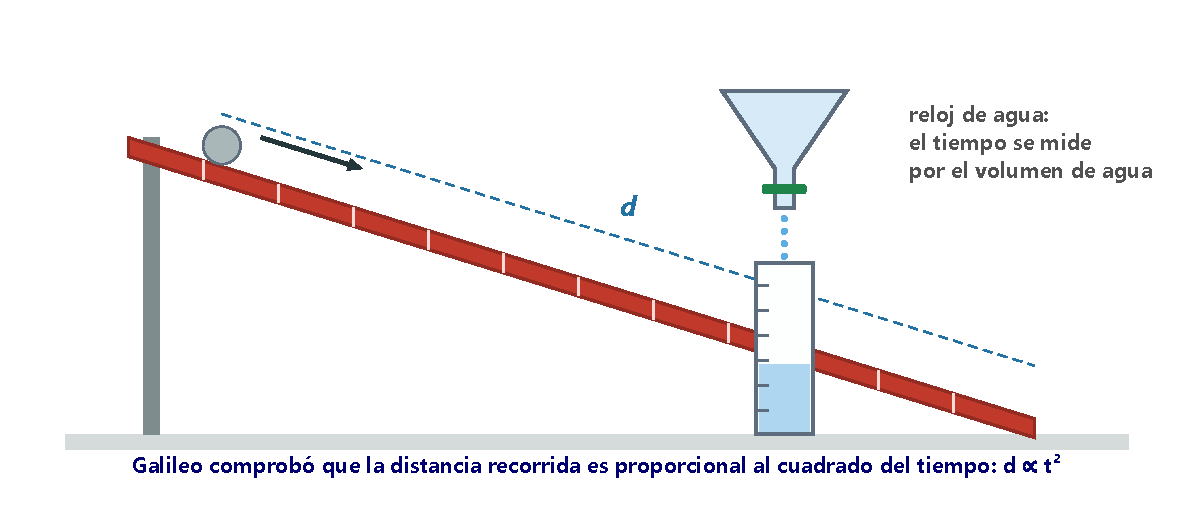
\includegraphics[width=0.6\textwidth]{images/UD9/plano_galileo}
    \caption{Reconstrucción del experimento de Galileo con el plano inclinado.}
    \label{fig:ud9-galileo}
\end{figure}

\begin{example}
    \textbf{Frenada.} Un conductor frena durante \qty{15}{\s} y recorre \qty{180}{\m} hasta pararse. Calcula: a) la velocidad que
    llevaba; b) la aceleración de frenado.

    \textbf{Solución.} Datos: \(t = \qty{15}{\s}\), \(\Delta x = \qty{180}{\m}\), \(v = 0\). Con las dos ecuaciones del MRUA:
    \[ 0 = v_0 + 15\,a \qquad\qquad 180 = 15\,v_0 + \frac{1}{2}\,a \cdot 15^2 \]
    De la primera, \(v_0 = -15\,a\); sustituyendo en la segunda, \(180 = -225\,a + \num{112.5}\,a = -\num{112.5}\,a\), de donde
    \(a = \qty{-1.6}{\m\per\s\squared}\) y \(v_0 = \qty{24}{\m\per\s}\) (\qty{86.4}{\km\per\hour}). (También se puede usar la
    velocidad media: \(v_m = \dfrac{v_0 + 0}{2} = \dfrac{180}{15} = \qty{12}{\m\per\s}\), así que \(v_0 = \qty{24}{\m\per\s}\).)
\end{example}

\begin{example}
    \textbf{¿Quién llega antes al autobús?} Marta corre hacia la parada del autobús, que está \qty{36}{\m} por delante de ella, a
    \qty{3}{\m\per\s} constantes. Su hermano Pablo, que está \qty{8}{\m} por detrás de ella, sale \qty{2}{\s} más tarde, desde el
    reposo, con una aceleración de \qty{1.2}{\m\per\s\squared}. a) ¿Quién llega antes a la parada? b) ¿A qué velocidad debería
    correr Marta para llegar a la vez que Pablo?

    \textbf{Solución.} Tomamos el origen en la posición inicial de Marta y \(t = 0\) cuando ella empieza a correr:
    \[ x_M = 3t \qquad\qquad x_P = -8 + \frac{1}{2} \cdot \num{1.2}\,(t - 2)^2 = -8 + \num{0.6}\,(t - 2)^2 \]
    a) Marta llega cuando \(3t = 36\): \(t = \qty{12}{\s}\). Pablo, cuando \(-8 + \num{0.6}(t - 2)^2 = 36\):
    \((t - 2)^2 = \num{73.3}\), \(t - 2 = \qty{8.56}{\s}\), \(t = \qty{10.56}{\s}\). \textbf{Pablo llega antes}, aunque salió más
    tarde y más lejos.

    b) Marta tendría que recorrer \qty{36}{\m} en \qty{10.56}{\s}: \(v = \dfrac{36}{\num{10.56}} = \qty{3.41}{\m\per\s}\).
\end{example}

\begin{exercise}
    Un móvil circula a \qty{20}{\m\per\s} y acelera a razón de \qty{4}{\m\per\s\squared}. Calcula: a) la velocidad y el espacio
    recorrido \qty{5}{\s} más tarde; b) la velocidad que tendrá cuando haya recorrido \qty{400}{\m}.
    \begin{solu}
        a) \(v = 20 + 4 \cdot 5 = \textcolor{red}{\qty{40}{\m\per\s}}\); \(\Delta x = 20 \cdot 5 + 2 \cdot 25 = \textcolor{red}{\qty{150}{\m}}\).
        b) \(v^2 = 400 + 2 \cdot 4 \cdot 400 = 3600\): \(\textcolor{red}{v = \qty{60}{\m\per\s}}\).
    \end{solu}
\end{exercise}

\begin{exercise}
    Villa Arriba y Villa Abajo están separadas por un camino recto de \qty{200}{\m}. Luis sale de Villa Abajo hacia Villa Arriba
    a \qty{4}{\m\per\s} y, como quiere llegar antes, acelera a \qty{0.5}{\m\per\s\squared}. A la vez, Ana sale de Villa Arriba
    hacia Villa Abajo a \qty{6}{\m\per\s} constantes. a) Escribe las ecuaciones de los dos movimientos y dibuja sus gráficas
    \(x\)-\(t\) y \(v\)-\(t\). b) ¿Cuándo y dónde se cruzan?
    \begin{solu}
        a) \textcolor{red}{\(x_L = 4t + 0{,}25\,t^2\); \(x_A = 200 - 6t\)}; \(v_L = 4 + 0{,}5\,t\) (recta creciente) y \(v_A = -6\)
        (recta horizontal). b) \(0{,}25\,t^2 + 10t - 200 = 0\): \(\textcolor{red}{t = \qty{14.6}{\s}}\), a
        \(\textcolor{red}{\qty{112}{\m}}\) de Villa Abajo.
    \end{solu}
\end{exercise}

\subsection{Movimiento vertical: caída libre}

Si dejamos caer o lanzamos un cuerpo en vertical y el rozamiento con el aire es despreciable, el cuerpo se mueve solo bajo la acción
de la gravedad: es un \textbf{movimiento de caída libre}, un caso particular de MRUA cuya aceleración es la \textbf{aceleración de la
gravedad}, \(\vec g\).

\begin{definition}[Aceleración de la gravedad]
    Cerca de la superficie terrestre, todos los cuerpos en caída libre tienen la misma aceleración, \(\vec g\), dirigida hacia el
    centro de la Tierra y de módulo \(g = \qty{9.8}{\m\per\s\squared}\), sea cual sea su masa.
\end{definition}

Tomamos el eje Y vertical y hacia arriba, con el origen en el suelo. Como \(\vec g\) apunta hacia abajo, \(a = -g\), y las ecuaciones
del MRUA quedan:
\[ \boxed{v_y = v_{0y} - g\,t} \qquad\qquad \boxed{y = y_0 + v_{0y}\,t - \frac{1}{2}\,g\,t^2} \qquad\qquad v_y^2 = v_{0y}^2 - 2\,g\,(y - y_0) \]
El signo negativo de \(g\) en las ecuaciones no depende de que el cuerpo suba o baje: la gravedad siempre tira hacia abajo.

\begin{itemize}
    \item \textbf{Se deja caer} (\(v_{0y} = 0\)) o \textbf{se lanza hacia abajo} (\(v_{0y} < 0\)): la velocidad es negativa durante
    toda la caída y su módulo aumenta.
    \item \textbf{Se lanza hacia arriba} (\(v_{0y} > 0\)), desde el suelo o desde cierta altura: \(v_y\) es positiva mientras sube,
    se anula en el punto más alto y es negativa mientras baja.
\end{itemize}

\textbf{Altura máxima.} En el punto más alto, \(v_y = 0\). El tiempo de subida se obtiene de \(0 = v_{0y} - g\,t_s\), es decir,
\(t_s = \dfrac{v_{0y}}{g}\), y la altura máxima, sustituyéndolo en la ecuación de la posición (o con
\(y_{\text{máx}} = y_0 + \dfrac{v_{0y}^2}{2g}\)). Si el cuerpo vuelve al mismo nivel desde el que se lanzó, tarda lo mismo en bajar que
en subir y llega con la misma rapidez con la que salió.

\begin{figure}[H]
    \centering
    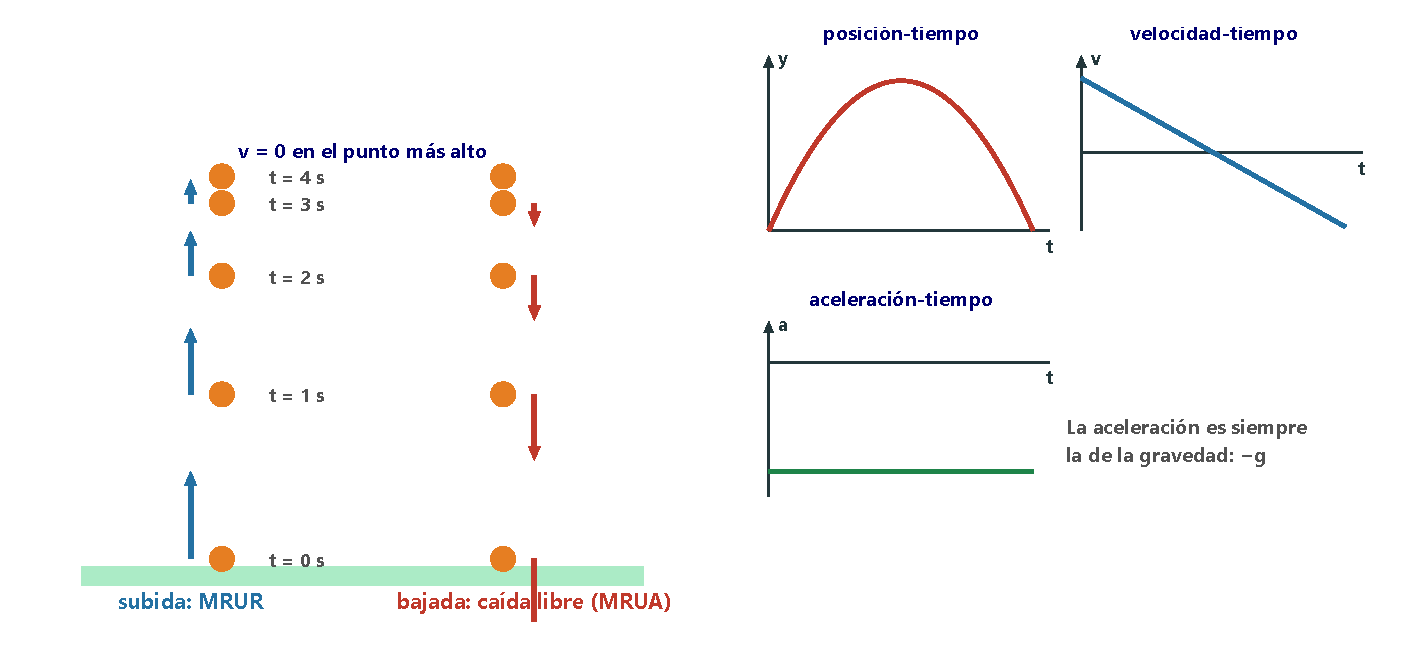
\includegraphics[width=0.95\textwidth]{images/UD9/lanzamiento_vertical}
    \caption{Lanzamiento vertical hacia arriba: subida con movimiento retardado, \(v = 0\) en el punto más alto, y bajada en caída
    libre. La aceleración es siempre \(-g\).}
    \label{fig:ud9-vertical}
\end{figure}

\begin{example}
    \textbf{Lanzamiento hacia arriba.} Pedro lanza una pelota hacia arriba a \qty{8}{\m\per\s}. Calcula: a) la altura máxima;
    b) el tiempo que está en el aire; c) la velocidad con la que vuelve a su mano.

    \textbf{Solución.} Origen en la mano: \(y = 8t - \num{4.9}\,t^2\) y \(v = 8 - \num{9.8}\,t\).
    a) En el punto más alto, \(v = 0\): \(t_s = \dfrac{8}{\num{9.8}} = \qty{0.816}{\s}\);
    \(y_{\text{máx}} = 8 \cdot \num{0.816} - \num{4.9} \cdot \num{0.816}^2 = \qty{3.27}{\m}\).
    b) Vuelve a \(y = 0\): \(t(8 - \num{4.9}\,t) = 0\), así que \(t = \qty{1.63}{\s}\), el doble del tiempo de subida.
    c) \(v = 8 - \num{9.8} \cdot \num{1.63} = \qty{-8}{\m\per\s}\): la misma rapidez, hacia abajo.
\end{example}

\begin{example}
    \textbf{Una herramienta desde un andamio.} Un andamio eléctrico sube a \qty{2}{\m\per\s} y, cuando está a \qty{30}{\m} de
    altura, se le cae una herramienta. Calcula: a) las ecuaciones de la posición y de la velocidad de la herramienta; b) cuánto tarda
    en llegar al suelo y con qué velocidad.

    \textbf{Solución.} a) La herramienta sale con la velocidad del andamio, \(v_0 = +\qty{2}{\m\per\s}\) (¡hacia arriba!):
    \(y = 30 + 2t - \num{4.9}\,t^2\) y \(v = 2 - \num{9.8}\,t\).
    b) Llega al suelo cuando \(y = 0\): \(\num{4.9}\,t^2 - 2t - 30 = 0\), con solución positiva \(t = \qty{2.69}{\s}\) (la negativa
    no tiene sentido físico). Entonces \(v = 2 - \num{9.8} \cdot \num{2.69} = \qty{-24.3}{\m\per\s}\): cae a \qty{24.3}{\m\per\s}.
\end{example}

\begin{example}
    \textbf{Encuentro en vertical.} Desde el suelo se lanza una llave hacia arriba a \qty{20}{\m\per\s} y, en el mismo instante, desde
    \qty{45}{\m} de altura se lanza una cerradura hacia abajo a \qty{8}{\m\per\s}. Calcula: a) cuándo y a qué altura se cruzan;
    b) dónde está la cerradura cuando la llave alcanza su altura máxima.

    \textbf{Solución.} \(y_1 = 20t - \num{4.9}\,t^2\) e \(y_2 = 45 - 8t - \num{4.9}\,t^2\).
    a) \(y_1 = y_2\): \(20t = 45 - 8t\) (¡los términos de \(t^2\) se anulan!), \(t = \qty{1.61}{\s}\), a una altura
    \(y = 20 \cdot \num{1.61} - \num{4.9} \cdot \num{1.61}^2 = \qty{19.5}{\m}\).
    b) La llave sube durante \(t = 20/\num{9.8} = \qty{2.04}{\s}\); entonces \(y_2 = 45 - 8 \cdot \num{2.04} - \num{4.9} \cdot
    \num{2.04}^2 = \qty{8.3}{\m}\): la cerradura todavía no ha llegado al suelo.
\end{example}

\begin{exercise}
    Se lanza un bolígrafo desde una ventana que está a \qty{25}{\m} de altura y tarda \qty{4}{\s} en llegar al suelo. ¿Con qué
    velocidad y en qué sentido se lanzó? Resuélvelo: a) tomando el origen en el suelo; b) tomando el origen en la ventana.
    \begin{solu}
        a) \(0 = 25 + 4\,v_0 - \num{4.9} \cdot 16\): \(\textcolor{red}{v_0 = \qty{13.4}{\m\per\s}}\), \textcolor{red}{hacia arriba}.
        b) \(-25 = 4\,v_0 - \num{78.4}\): el mismo resultado. El origen no cambia la física.
    \end{solu}
\end{exercise}

\begin{exercise}
    Desde lo alto de una torre de \qty{40}{\m} se lanza una caja verticalmente hacia arriba a \qty{10}{\m\per\s}. Calcula: a) su
    velocidad y su altura a los \qty{2}{\s}; b) la altura máxima y el tiempo que tarda en alcanzarla.
    \begin{solu}
        a) \(v = 10 - \num{19.6} = \textcolor{red}{\qty{-9.6}{\m\per\s}}\) (ya baja); \(y = 40 + 20 - \num{19.6} = \textcolor{red}{\qty{40.4}{\m}}\).
        b) \(\textcolor{red}{t = \qty{1.02}{\s}}\); \(y_{\text{máx}} = 40 + \dfrac{100}{\num{19.6}} = \textcolor{red}{\qty{45.1}{\m}}\).
    \end{solu}
\end{exercise}

%========================================================================================
\section{Composición de movimientos}\label{sec:ud9-composicion}
%========================================================================================

Muchos movimientos son la combinación de otros más sencillos: un kayak que cruza un río, una persona que camina por la cinta de un
aeropuerto o un balón lanzado a canasta. Para estudiarlos se usa una idea que ya aplicaba Galileo en el siglo \textsc{xvii}:

\begin{definition}[Principio de superposición]
    Cuando un cuerpo está sometido a varios movimientos simultáneos e independientes, el movimiento resultante se obtiene
    \textbf{sumando vectorialmente} las posiciones, velocidades y aceleraciones de cada uno de ellos, como si cada movimiento parcial
    ocurriera por separado. El \textbf{tiempo} es el mismo para todos los movimientos componentes.
\end{definition}

\subsection{Movimientos de la misma dirección}

Si los movimientos tienen la misma dirección, basta con sumar las velocidades con su signo:
\begin{itemize}
    \item \textbf{Dos MRU} dan un \textbf{MRU}, en el sentido del más rápido. Ejemplos: una persona que camina por una cinta
    transportadora o un salmón que remonta un río.
    \item Si \textbf{alguno es un MRUA}, el movimiento resultante es un \textbf{MRUA}. Ejemplo: un objeto que se deja caer dentro de
    un ascensor que sube con velocidad constante, visto desde fuera.
\end{itemize}

\begin{example}
    \textbf{En el aeropuerto.} Identifica el tipo de composición: a) arrancas a correr sobre una cinta transportadora para no perder
    el avión; b) nadas a \qty{1.2}{\m\per\s} a favor de la corriente de un río que fluye a \qty{0.5}{\m\per\s}.

    \textbf{Solución.} a) La cinta tiene un MRU y tú, sobre ella, un MRUA (arrancas desde el reposo): el resultado es un
    \textbf{MRUA}. b) Las dos velocidades son constantes y del mismo sentido: un \textbf{MRU} a \(\num{1.2} + \num{0.5} =
    \qty{1.7}{\m\per\s}\) respecto a la orilla.
\end{example}

\begin{exercise}
    a) Una pulga camina con rapidez constante sobre la cabeza de un perro que corre de forma uniforme por un sendero. b) En un globo
    aerostático que asciende con velocidad constante, juegas a lanzar una pelota hacia arriba y recogerla. Explica qué tipo de
    composición observa en cada caso una persona en reposo en el suelo.
    \begin{solu}
        a) \textcolor{red}{MRU + MRU = MRU}. b) \textcolor{red}{MRU (globo) + MRUA (pelota) = MRUA}: para la persona del suelo, la
        pelota sale con más velocidad (la suya más la del globo), pero su aceleración sigue siendo \(-g\).
    \end{solu}
\end{exercise}

\subsection{Movimientos perpendiculares}

\subsubsection{Composición de dos MRU: cruzar un río}

Una barca cruza un río remando con velocidad constante \(\vec v_n\) perpendicular a la orilla, mientras la corriente la arrastra con
velocidad \(\vec v_c\), también constante. Tomamos el eje X en la dirección de la corriente y el eje Y perpendicular a la orilla:
\[ x = v_c\,t \qquad y = v_n\,t \qquad \vec v = v_c\,\ivec + v_n\,\jvec \qquad |\vec v| = \sqrt{v_c^2 + v_n^2} \]
\begin{itemize}
    \item El \textbf{tiempo} que tarda en cruzar depende solo de la componente perpendicular: \(t = \dfrac{\text{anchura}}{v_n}\).
    La corriente no la retrasa.
    \item En ese tiempo, la corriente la arrastra río abajo una distancia \(x = v_c\,t\).
    \item La trayectoria es una recta, \(y = \dfrac{v_n}{v_c}\,x\), que forma con la corriente un ángulo \(\alpha\) tal que
    \(\tg\alpha = \dfrac{v_n}{v_c}\).
\end{itemize}

\begin{figure}[H]
    \centering
    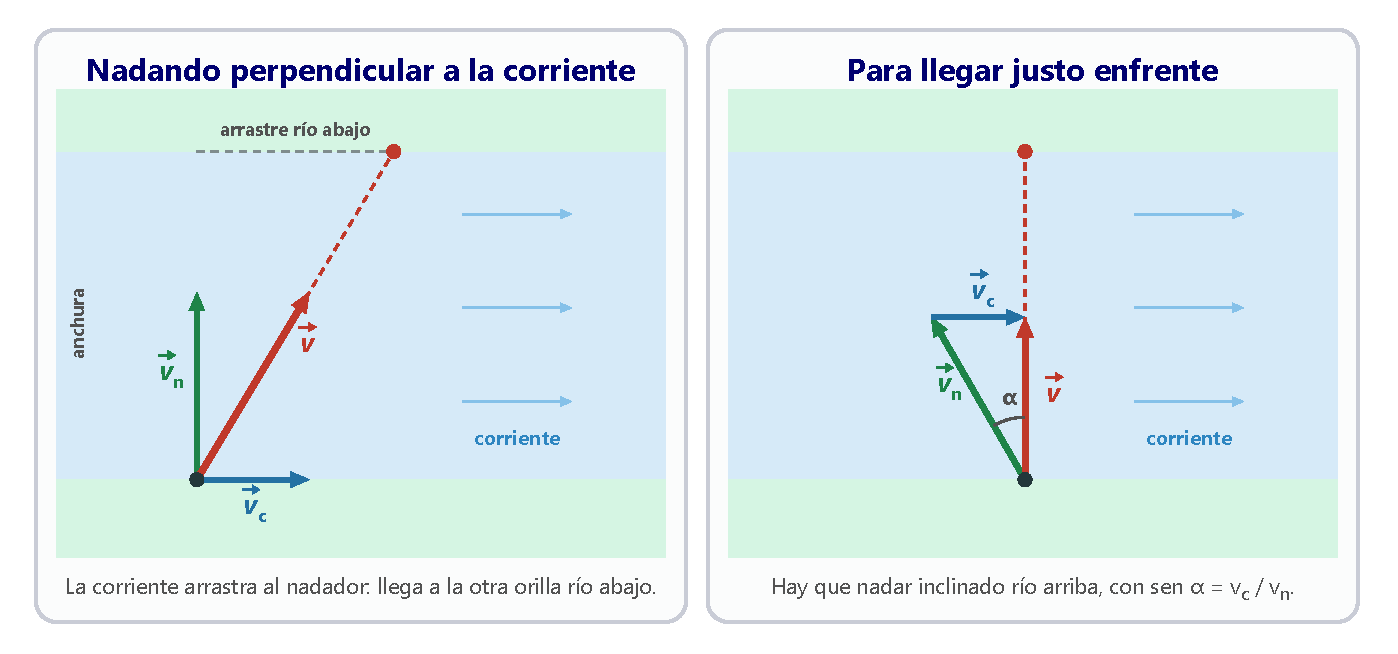
\includegraphics[width=0.9\textwidth]{images/UD9/composicion_rio}
    \caption{Composición de dos MRU perpendiculares: la velocidad real es la suma vectorial de la propia y la de la corriente.}
    \label{fig:ud9-rio}
\end{figure}

\begin{example}
    \textbf{Llegar justo enfrente.} Un río de \qty{24}{\m} de ancho lleva una corriente de \qty{2}{\m\per\s}. Un nadador puede
    nadar a \qty{4}{\m\per\s} respecto al agua. ¿En qué dirección debe nadar para llegar justo enfrente? ¿Cuánto tardará?

    \textbf{Solución.} Debe nadar inclinado río arriba, de modo que la componente de su velocidad paralela a la orilla anule la
    corriente (figura~\ref{fig:ud9-rio}, derecha). Si \(\alpha\) es el ángulo con la perpendicular a la orilla:
    \[ \sen\alpha = \frac{v_c}{v_n} = \frac{2}{4} = \num{0.5} \quad\Rightarrow\quad \alpha = 30^\circ \text{ río arriba} \]
    Su velocidad real es perpendicular a la orilla, de módulo \(v = \sqrt{4^2 - 2^2} = \qty{3.46}{\m\per\s}\), y tarda
    \(t = \dfrac{24}{\num{3.46}} = \qty{6.93}{\s}\).
\end{example}

\begin{exercise}
    Se quiere cruzar un río de \qty{40}{\m} de ancho nadando a \qty{2}{\m\per\s} perpendicularmente a una corriente de
    \qty{1.2}{\m\per\s}. Calcula: a) la velocidad real del nadador respecto a la orilla; b) el ángulo que forma con la corriente;
    c) el tiempo que tarda en llegar a la otra orilla; d) la distancia que lo arrastra la corriente.
    \begin{solu}
        a) \(\sqrt{4 + \num{1.44}} = \textcolor{red}{\qty{2.33}{\m\per\s}}\); b) \(\tg\alpha = \dfrac{2}{\num{1.2}}\):
        \(\textcolor{red}{\alpha = 59^\circ}\); c) \(\dfrac{40}{2} = \textcolor{red}{\qty{20}{\s}}\); d) \(\num{1.2} \cdot 20 =
        \textcolor{red}{\qty{24}{\m}}\) río abajo.
    \end{solu}
\end{exercise}

\subsubsection{Tiro parabólico: composición de un MRU y un MRUA}

\begin{definition}[Tiro parabólico u oblicuo]
    Es el movimiento de un cuerpo lanzado con una velocidad inicial \(\vec v_0\) que forma un ángulo \(\alpha\) con la horizontal y que
    se mueve después solo bajo la acción de la gravedad (despreciamos el rozamiento con el aire). Su trayectoria es una
    \textbf{parábola}.
\end{definition}

Ejemplos: el saque de un balón de voleibol, un golpe de golf o el salto de una moto en una rampa. Descomponemos la velocidad inicial
en una componente horizontal y otra vertical:
\[ v_{0x} = v_0\cos\alpha \qquad\qquad v_{0y} = v_0\,\sen\alpha \]
\begin{itemize}
    \item En el eje X no hay aceleración: el movimiento horizontal es un \textbf{MRU} con velocidad \(v_{0x}\), que produce el avance.
    \item En el eje Y la aceleración es \(-g\): el movimiento vertical es un \textbf{MRUA} (un lanzamiento vertical) con velocidad
    inicial \(v_{0y}\), que produce la subida y la bajada.
\end{itemize}

\begin{figure}[H]
    \centering
    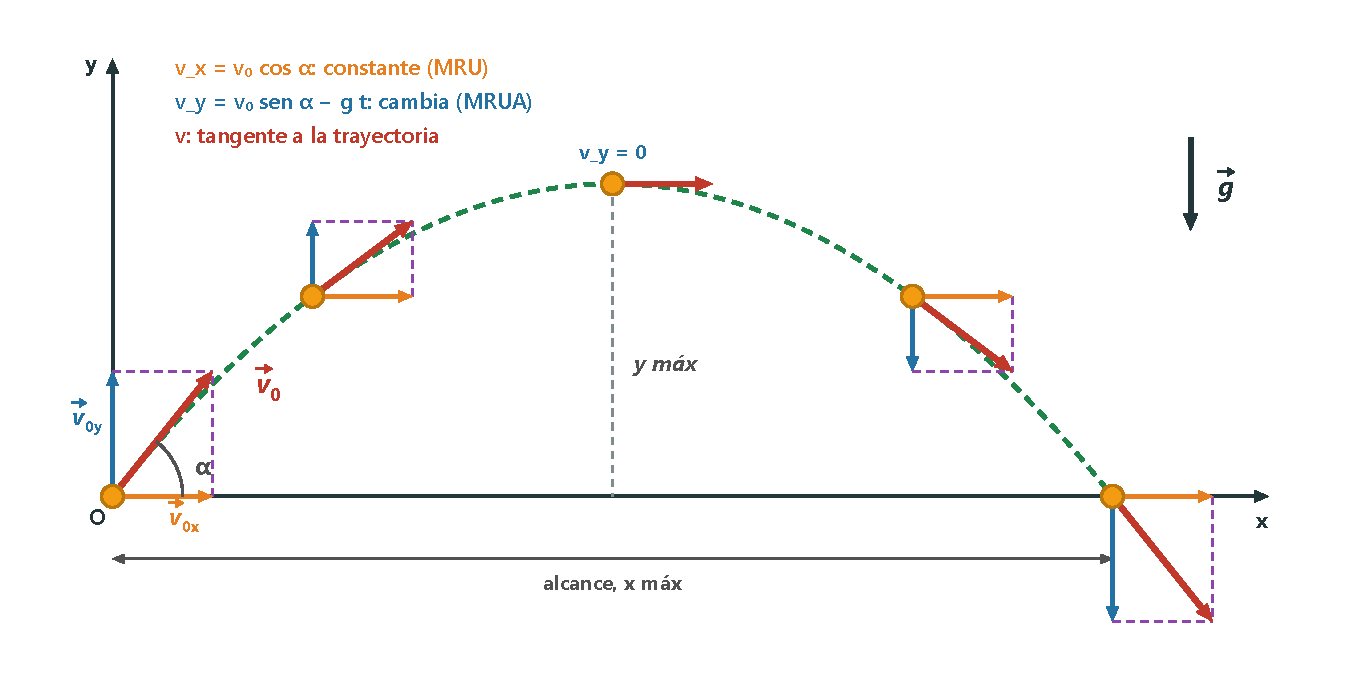
\includegraphics[width=0.95\textwidth]{images/UD9/tiro_parabolico}
    \caption{En el tiro parabólico, la componente horizontal de la velocidad es constante y la vertical cambia como en un lanzamiento
    vertical.}
    \label{fig:ud9-parabolico}
\end{figure}

Con el origen en el suelo, en la vertical del punto de lanzamiento, y la posición inicial \((0, y_0)\):

\begin{table}[H]
    \centering
    \caption{Ecuaciones del tiro parabólico}
    \vspace{-5pt}
    \begin{tabular}{@{}lL{9cm}@{}}
        \toprule
        \textbf{Magnitud} & \textbf{Ecuación} \\
        \midrule
        Posición & \(x = v_0\cos\alpha\,t\) \qquad \(y = y_0 + v_0\,\sen\alpha\,t - \frac{1}{2}\,g\,t^2\) \\[3pt]
        Velocidad & \(v_x = v_0\cos\alpha\) (constante) \qquad \(v_y = v_0\,\sen\alpha - g\,t\) \\[3pt]
        Vectores & \(\vec r = x\,\ivec + y\,\jvec\) \qquad \(\vec v = v_x\,\ivec + v_y\,\jvec\) \qquad \(\vec a = -g\,\jvec\) \\[3pt]
        Trayectoria & \(y = y_0 + x\,\tg\alpha - \dfrac{g}{2\,v_0^2\cos^2\alpha}\,x^2\) (una parábola) \\
        \bottomrule
    \end{tabular}
    \label{tab:ud9-parabolico}
\end{table}

Tres magnitudes caracterizan el lanzamiento:
\begin{itemize}
    \item \textbf{Tiempo de vuelo}: el que tarda en llegar al suelo, cuando \(y = 0\). Si se lanzó desde el suelo (\(y_0 = 0\)):
    \(t_{\text{vuelo}} = \dfrac{2\,v_0\,\sen\alpha}{g}\).
    \item \textbf{Altura máxima}: en ella, \(v_y = 0\). Desde el suelo: \(y_{\text{máx}} = \dfrac{v_0^2\,\sen^2\alpha}{2g}\).
    \item \textbf{Alcance}: la distancia horizontal recorrida hasta tocar el suelo, \(x_{\text{máx}} = v_0\cos\alpha\,t_{\text{vuelo}}\).
    Desde el suelo: \(x_{\text{máx}} = \dfrac{v_0^2\,\sen 2\alpha}{g}\). El alcance es máximo para \(\alpha = 45^\circ\), y dos
    ángulos complementarios (\(30^\circ\) y \(60^\circ\), por ejemplo) dan el mismo alcance.
\end{itemize}
Si el cuerpo se lanza desde cierta altura o choca con un obstáculo, no se pueden usar estas fórmulas abreviadas: hay que plantear las
ecuaciones de la tabla~\ref{tab:ud9-parabolico}.

\begin{example}
    \textbf{Un proyectil.} Se lanza un proyectil desde el suelo a \qty{80}{\m\per\s} con una inclinación de \(35^\circ\) sobre la
    horizontal. Despreciando el rozamiento con el aire, calcula: a) la altura máxima; b) a qué distancia horizontal del punto de
    lanzamiento la alcanza; c) el alcance.

    \textbf{Solución.} Componentes de la velocidad inicial: \(v_{0x} = 80\cos 35^\circ = \qty{65.5}{\m\per\s}\) y
    \(v_{0y} = 80\,\sen 35^\circ = \qty{45.9}{\m\per\s}\). Ecuaciones: \(x = \num{65.5}\,t\); \(y = \num{45.9}\,t - \num{4.9}\,t^2\);
    \(v_y = \num{45.9} - \num{9.8}\,t\).

    a) En el punto más alto, \(v_y = 0\): \(t = \dfrac{\num{45.9}}{\num{9.8}} = \qty{4.68}{\s}\), y
    \(y_{\text{máx}} = \num{45.9} \cdot \num{4.68} - \num{4.9} \cdot \num{4.68}^2 = \qty{107}{\m}\).
    b) \(x = \num{65.5} \cdot \num{4.68} = \qty{307}{\m}\).
    c) Llega al suelo cuando \(y = 0\): \(t(\num{45.9} - \num{4.9}\,t) = 0\), \(t = \qty{9.36}{\s}\) (el doble que la subida), y
    \(x_{\text{máx}} = \num{65.5} \cdot \num{9.36} = \qty{614}{\m}\). Con la fórmula: \(\dfrac{80^2\,\sen 70^\circ}{\num{9.8}} =
    \qty{614}{\m}\).
\end{example}

\begin{exercise}
    Andrea juega al golf y está a \qty{250}{\m} del hoyo. Va a golpear la pelota con un ángulo de \(30^\circ\) con la horizontal.
    a) ¿Con qué velocidad debe salir la pelota para caer en el hoyo? b) ¿Cuánto tiempo estará en el aire?
    \begin{solu}
        a) \(250 = \dfrac{v_0^2\,\sen 60^\circ}{\num{9.8}}\): \(\textcolor{red}{v_0 = \qty{53.2}{\m\per\s}}\).
        b) \(t = \dfrac{2 \cdot \num{53.2} \cdot \sen 30^\circ}{\num{9.8}} = \textcolor{red}{\qty{5.43}{\s}}\).
    \end{solu}
\end{exercise}

\begin{exercise}
    Una futbolista lanza una falta a \qty{25}{\m\per\s} con un ángulo de \(25^\circ\). Si el balón no tocara a nadie ni la portería,
    ¿cuánto tiempo estaría en el aire? ¿A qué distancia caería? ¿Qué altura máxima alcanzaría?
    \begin{solu}
        \(t = \dfrac{2 \cdot 25\,\sen 25^\circ}{\num{9.8}} = \textcolor{red}{\qty{2.16}{\s}}\); \(x = \dfrac{625\,\sen 50^\circ}{\num{9.8}} =
        \textcolor{red}{\qty{48.9}{\m}}\); \(y_{\text{máx}} = \dfrac{625\,\sen^2 25^\circ}{\num{19.6}} = \textcolor{red}{\qty{5.70}{\m}}\).
    \end{solu}
\end{exercise}

\begin{exercise}
    Con un laboratorio virtual de tiro parabólico (o con las fórmulas), completa estas tablas y saca conclusiones. a) Con \(\alpha =
    45^\circ\), calcula el alcance para \(v_0 = 5\), 8, 11, 14, 17 y \qty{20}{\m\per\s}. b) Con \(v_0 = \qty{15}{\m\per\s}\), calcula el
    alcance para \(\alpha = 25^\circ\), \(35^\circ\), \(45^\circ\), \(55^\circ\), \(65^\circ\) y \(75^\circ\).
    \begin{solu}
        a) \(x = v_0^2/g\): \textcolor{red}{2,55; 6,53; 12,3; 20,0; 29,5 y \qty{40.8}{\m}}: \textcolor{red}{el alcance es proporcional
        al cuadrado de la velocidad}. b) \(x = 225\,\sen 2\alpha/\num{9.8}\): \textcolor{red}{17,6; 21,6; 23,0; 21,6; 17,6 y
        \qty{11.5}{\m}}: \textcolor{red}{máximo a \(45^\circ\); ángulos complementarios dan el mismo alcance}.
    \end{solu}
\end{exercise}

\subsubsection{Tiro horizontal}

\begin{definition}[Tiro horizontal]
    Es el movimiento de un cuerpo lanzado desde una altura \(y_0\) con una velocidad inicial \(\vec v_0\) \textbf{horizontal}. Es el
    caso particular del tiro parabólico con \(\alpha = 0\): \(v_{0x} = v_0\) y \(v_{0y} = 0\).
\end{definition}

Ejemplos: una gota de rocío que se desliza por una hoja y cae, o un paquete de ayuda humanitaria que se suelta desde un avión que
vuela en horizontal. Las ecuaciones son:
\[ x = v_0\,t \qquad y = y_0 - \frac{1}{2}\,g\,t^2 \qquad v_x = v_0 \qquad v_y = -g\,t \qquad
   \text{trayectoria: } y = y_0 - \frac{g}{2\,v_0^2}\,x^2 \]

\begin{figure}[H]
    \centering
    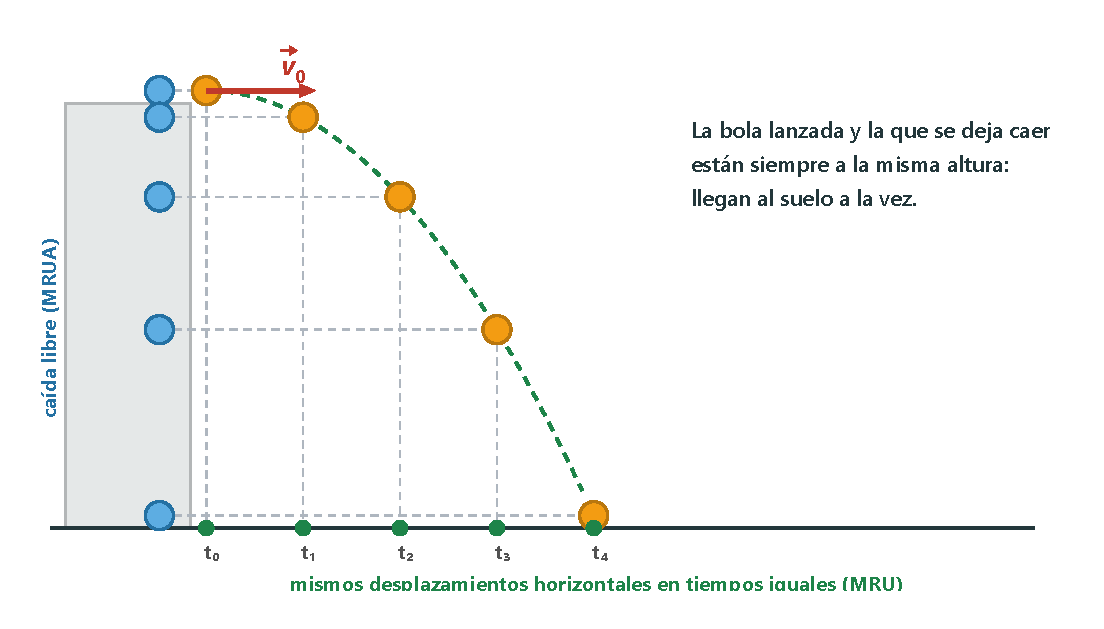
\includegraphics[width=0.75\textwidth]{images/UD9/tiro_horizontal}
    \caption{Una bola lanzada horizontalmente y otra que se deja caer a la vez desde la misma altura llegan juntas al suelo.}
    \label{fig:ud9-horizontal}
\end{figure}

\begin{remark}
    \textbf{Todos llegan a la vez.} El lanzamiento vertical, el horizontal y el parabólico son movimientos de caída libre. Por eso, los
    cuerpos que caen desde la misma altura máxima tardan exactamente lo mismo en llegar al suelo, tanto si se dejan caer como si se
    lanzan horizontalmente: el movimiento horizontal no influye en el vertical.
\end{remark}

\begin{example}
    \textbf{La flecha y la manzana.} Un arquero lanza una flecha horizontalmente desde un puente de \qty{20}{\m} de altura a
    \qty{12}{\m\per\s}, y en el mismo instante se deja caer una manzana desde el mismo puente. Despreciando el rozamiento, calcula:
    a) el tiempo que la flecha está en el aire; b) a qué distancia del puente cae; c) su velocidad y su ángulo al llegar al agua;
    d) ¿cuál llega antes al agua y cuál lo hace más rápido?

    \textbf{Solución.} Flecha: \(x = 12t\); \(y = 20 - \num{4.9}\,t^2\); \(v_x = 12\); \(v_y = -\num{9.8}\,t\).
    a) \(y = 0\): \(t = \sqrt{\dfrac{20}{\num{4.9}}} = \qty{2.02}{\s}\). b) \(x = 12 \cdot \num{2.02} = \qty{24.2}{\m}\).
    c) \(v_y = -\num{9.8} \cdot \num{2.02} = \qty{-19.8}{\m\per\s}\); \(\vec v = (12\,\ivec - \num{19.8}\,\jvec)~\unit{\m\per\s}\), de módulo
    \(\sqrt{144 + 392} = \qty{23.2}{\m\per\s}\). El ángulo con la horizontal es \(\alpha = \arctg\dfrac{\num{19.8}}{12} = 58.8^\circ\),
    por debajo de ella.
    d) La manzana cumple \(y = 20 - \num{4.9}\,t^2\), igual que la flecha: \textbf{llegan a la vez}. Pero la manzana llega a
    \qty{19.8}{\m\per\s}, más despacio que la flecha, porque no tiene componente horizontal.
\end{example}

\begin{exercise}
    a) Un pájaro que vuela horizontalmente a \qty{25}{\m\per\s} suelta una ramita. Escribe la velocidad de la ramita en función del
    tiempo. b) Desde un helicóptero que avanza horizontalmente a \qty{30}{\m\per\s} a \qty{150}{\m} de altura cae un objeto. Escribe
    su componente vertical de la posición, su vector posición y su componente vertical de la velocidad.
    \begin{solu}
        a) \(\textcolor{red}{\vec v = (25\,\ivec - \num{9.8}\,t\,\jvec)~\unit{\m\per\s}}\). b) \(\textcolor{red}{y = 150 - \num{4.9}\,t^2}\);
        \(\textcolor{red}{\vec r = 30t\,\ivec + (150 - \num{4.9}\,t^2)\,\jvec~\unit{\m}}\); \(\textcolor{red}{v_y = -\num{9.8}\,t~\unit{\m\per\s}}\).
    \end{solu}
\end{exercise}

\begin{exercise}
    Se lanza horizontalmente una pelota a \qty{8}{\m\per\s} desde \qty{25}{\m} de altura. Calcula: a) los vectores velocidad y
    posición; b) a qué distancia cae.
    \begin{solu}
        a) \(\textcolor{red}{\vec v = 8\,\ivec - \num{9.8}\,t\,\jvec}\); \(\textcolor{red}{\vec r = 8t\,\ivec + (25 - \num{4.9}\,t^2)\,\jvec}\).
        b) \(t = \sqrt{25/\num{4.9}} = \qty{2.26}{\s}\); \(x = \textcolor{red}{\qty{18.1}{\m}}\).
    \end{solu}
\end{exercise}

\begin{exercise}
    Joseba juega al pádel en una pista de \qty{20}{\m} de largo con la red, de \qty{0.88}{\m}, en el centro. Golpea la pelota
    horizontalmente a \qty{80}{\km\per\hour} desde el fondo de la pista y a \qty{1.9}{\m} de altura. a) ¿A qué altura llega la
    pelota a la red? ¿Pasa por encima? b) ¿Cuánto tiempo está en el aire y a qué distancia del fondo contrario bota?
    \begin{solu}
        a) \textcolor{blue}{\(v_0 = \qty{22.2}{\m\per\s}\); llega a la red (\(x = 10\)) en \(t = \qty{0.45}{\s}\).}
        \(y = \num{1.9} - \num{4.9} \cdot \num{0.45}^2 = \textcolor{red}{\qty{0.91}{\m}}\): \textcolor{red}{pasa por muy poco}.
        b) \(t = \sqrt{\num{1.9}/\num{4.9}} = \textcolor{red}{\qty{0.62}{\s}}\); \(x = \qty{13.8}{\m}\): bota a
        \(\textcolor{red}{\qty{6.2}{\m}}\) del fondo contrario.
    \end{solu}
\end{exercise}

%========================================================================================
\section{El movimiento circular}\label{sec:ud9-circular}
%========================================================================================

\begin{definition}[Movimiento circular]
    Un \textbf{movimiento circular} es aquel cuya trayectoria es una circunferencia.
\end{definition}

Son movimientos circulares los de las aspas de un aerogenerador, un tiovivo, la rueda de una jaula de hámster o un punto de un CD.
Conviene colocar el origen del sistema de referencia en el centro de la circunferencia: así, el módulo del vector posición es
siempre el radio \(R\) y solo cambia su dirección, que se describe con el ángulo \(\varphi\) que forma con el eje X. Por eso el
movimiento circular se describe muy bien con \textbf{magnitudes angulares}.

\subsection{Magnitudes angulares}

\begin{table}[H]
    \centering
    \caption{Magnitudes angulares del movimiento circular}
    \vspace{-5pt}
    \begin{tabular}{@{}lL{9.5cm}@{}}
        \toprule
        \textbf{Magnitud} & \textbf{Definición} \\
        \midrule
        Posición angular, \(\varphi\) & Ángulo que forma el vector posición con el semieje X positivo. Se mide en radianes (rad) \\[3pt]
        Desplazamiento angular, \(\Delta\varphi\) & Ángulo girado entre dos instantes: \(\Delta\varphi = \varphi - \varphi_0\) (rad) \\[3pt]
        Velocidad angular media, \(\omega_m\) & \(\omega_m = \dfrac{\Delta\varphi}{\Delta t}\), en \unit{\radian\per\s} \\[8pt]
        Velocidad angular, \(\omega\) & \(\omega = \dfrac{\dif\varphi}{\dif t}\), en \unit{\radian\per\s}. Es positiva en sentido antihorario y negativa en el horario \\[8pt]
        Aceleración angular, \(\alpha\) & \(\alpha = \dfrac{\dif\omega}{\dif t}\), en \unit{\radian\per\s\squared} \\
        \bottomrule
    \end{tabular}
    \label{tab:ud9-angulares}
\end{table}

\begin{figure}[H]
    \centering
    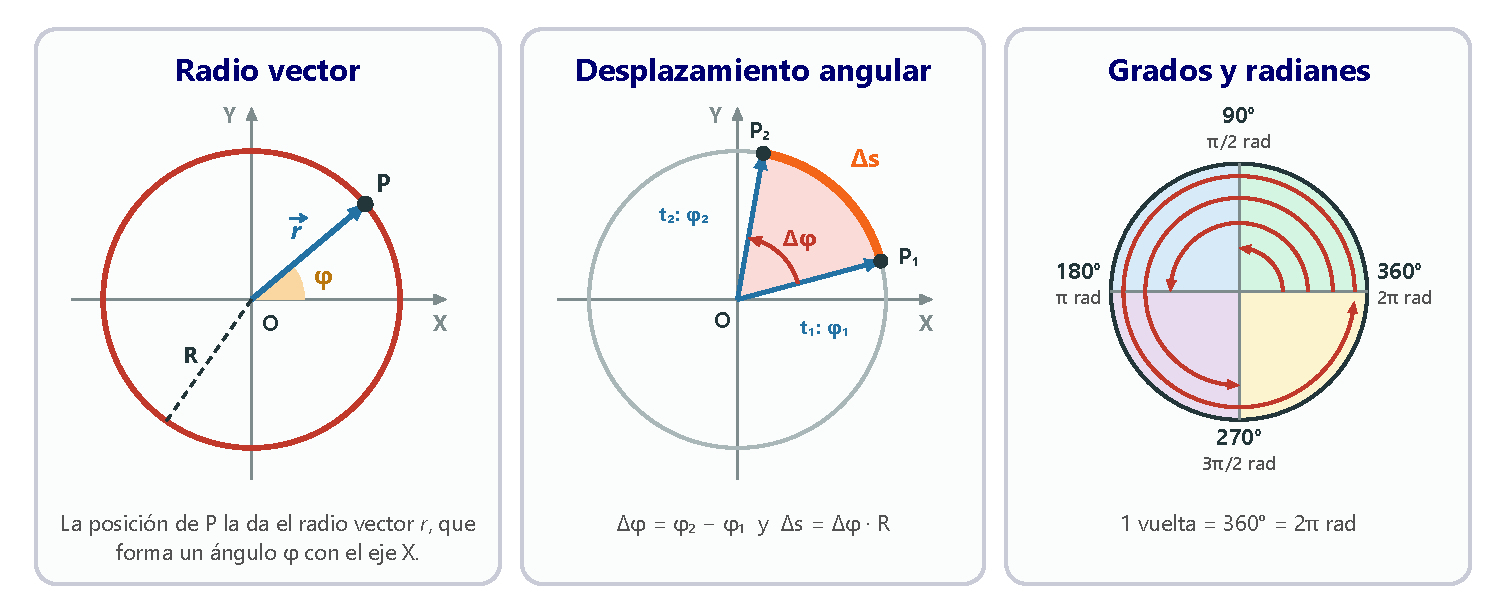
\includegraphics[width=0.95\textwidth]{images/UD9/mcu_magnitudes}
    \caption{Posición angular, desplazamiento angular y equivalencia entre grados y radianes.}
    \label{fig:ud9-angulares}
\end{figure}

\subsubsection{Relación entre las magnitudes angulares y las lineales}

El radio es el factor que relaciona las magnitudes angulares con las lineales (las medidas sobre la trayectoria):
\[ \Delta s = R\,\Delta\varphi \qquad\qquad v = R\,\omega \qquad\qquad a_t = R\,\alpha \]
Todos los puntos de un disco que gira tienen la misma velocidad angular, pero los más alejados del centro tienen más velocidad
lineal: recorren un arco más largo en el mismo tiempo.

\begin{figure}[H]
    \centering
    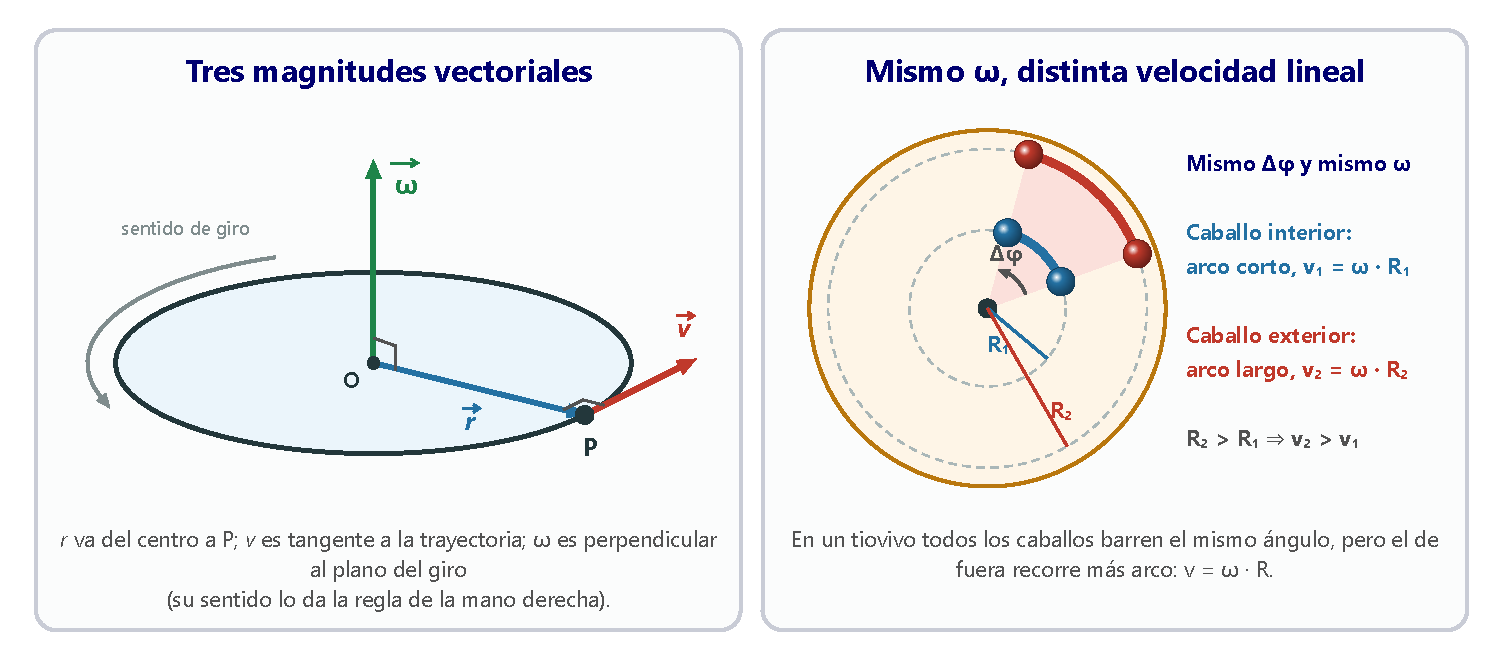
\includegraphics[width=0.95\textwidth]{images/UD9/mcu_vectores}
    \caption{En un tiovivo todos los caballos giran con la misma \(\omega\), pero los exteriores van más deprisa.}
    \label{fig:ud9-vectores}
\end{figure}

\begin{example}
    \textbf{Una plataforma giratoria.} Una plataforma de \qty{40}{\cm} de radio da 4 vueltas cada minuto. ¿Cuál es su velocidad
    angular? ¿Y la velocidad lineal de un punto del borde?

    \textbf{Solución.} \(\omega = 4~\dfrac{\text{vueltas}}{\unit{\minute}} \cdot \dfrac{2\pi~\text{rad}}{1~\text{vuelta}} \cdot
    \dfrac{\qty{1}{\minute}}{\qty{60}{\s}} = \dfrac{2\pi}{15} = \qty{0.419}{\radian\per\s}\);
    \(v = \omega\,R = \num{0.419} \cdot \num{0.40} = \qty{0.168}{\m\per\s}\).
\end{example}

\subsection{Movimiento circular uniforme (MCU)}

\begin{definition}[MCU]
    En el \textbf{movimiento circular uniforme} la trayectoria es una circunferencia y la rapidez es constante, es decir, la
    \textbf{velocidad angular \(\omega\) es constante}.
\end{definition}

Como \(\omega\) es constante, coincide con la media; despejando la posición angular (con \(t_0 = 0\)) obtenemos la ecuación del MCU:
\[ \boxed{\varphi = \varphi_0 + \omega\,t} \]
\begin{itemize}
    \item La rapidez es constante, así que \textbf{no hay aceleración tangencial}: \(a_t = 0\) y \(\alpha = 0\).
    \item La dirección de la velocidad cambia continuamente, así que \textbf{sí hay aceleración normal}, dirigida hacia el centro y
    de módulo constante: \(\boxed{a_n = \dfrac{v^2}{R} = \omega^2\,R}\).
\end{itemize}

\subsubsection{El MCU es periódico}

El MCU es un \textbf{movimiento periódico}: la posición, la velocidad y la aceleración se repiten cada vez que el móvil da una vuelta.
\begin{itemize}
    \item El \textbf{periodo}, \(T\), es el tiempo que tarda en dar una vuelta completa (en girar \(2\pi\)~rad). Se mide en segundos.
    \item La \textbf{frecuencia}, \(f\), es el número de vueltas por unidad de tiempo. Se mide en \unit{\per\s}, que se llama
    \textbf{hercio} (Hz).
\end{itemize}
\[ \boxed{T = \frac{2\pi}{\omega}} \qquad\qquad \boxed{f = \frac{1}{T} = \frac{\omega}{2\pi}} \]

\begin{remark}
    \textbf{Paralelismo entre los movimientos uniformes.} En el MRU, \(\Delta x = v\,t\) con \(v\) constante; en el MCU,
    \(\Delta s = v\,t\) con la rapidez constante y, en magnitudes angulares, \(\Delta\varphi = \omega\,t\) con \(\omega\) constante.
\end{remark}

\begin{example}
    \textbf{La Luna.} La Luna da una vuelta alrededor de la Tierra en \num{27.3} días, a una distancia media de
    \qty{3.84e8}{\m}. Suponiendo que su órbita es circular, calcula: a) su periodo en segundos, su frecuencia y su velocidad angular;
    b) su aceleración normal.

    \textbf{Solución.} a) \(T = \num{27.3}~\text{días} \cdot \dfrac{\qty{24}{\hour}}{1~\text{día}} \cdot \dfrac{\qty{3600}{\s}}{\qty{1}{\hour}} =
    \qty{2.36e6}{\s}\); \(f = \dfrac{1}{T} = \qty{4.24e-7}{\hertz}\); \(\omega = \dfrac{2\pi}{T} = \qty{2.66e-6}{\radian\per\s}\).
    b) \(a_n = \omega^2\,R = (\num{2.66e-6})^2 \cdot \num{3.84e8} = \qty{2.72e-3}{\m\per\s\squared}\), unas \num{3600} veces menor que
    \(g\): fue una de las pistas que llevaron a Newton a su ley de la gravitación.
\end{example}

\begin{exercise}
    Las palas de un aerogenerador miden \qty{30}{\m} y giran a 15 vueltas por minuto. Calcula: a) la velocidad angular, el periodo y
    la frecuencia; b) la velocidad lineal y la aceleración normal del extremo de una pala.
    \begin{solu}
        a) \(\textcolor{red}{\omega = \qty{1.57}{\radian\per\s}}\); \(\textcolor{red}{T = \qty{4}{\s}}\); \(\textcolor{red}{f = \qty{0.25}{\hertz}}\).
        b) \(v = \num{1.57} \cdot 30 = \textcolor{red}{\qty{47.1}{\m\per\s}}\) (\qty{170}{\km\per\hour}); \(a_n = \num{1.57}^2 \cdot 30 =
        \textcolor{red}{\qty{74.0}{\m\per\s\squared}}\).
    \end{solu}
\end{exercise}

\subsection{Movimiento circular uniformemente acelerado (MCUA)}

\begin{definition}[MCUA]
    En el \textbf{movimiento circular uniformemente acelerado} la trayectoria es una circunferencia y la \textbf{aceleración angular
    \(\alpha\) es constante}.
\end{definition}

Ahora cambian tanto la dirección como el módulo de la velocidad, así que hay los dos tipos de aceleración:
\begin{itemize}
    \item \textbf{aceleración tangencial}, constante: \(a_t = \alpha\,R\);
    \item \textbf{aceleración normal}, que crece o disminuye con la velocidad: \(a_n = \dfrac{v^2}{R} = \omega^2 R\).
\end{itemize}
Las ecuaciones del MCUA son las del MRUA cambiando las magnitudes lineales por las angulares (con \(t_0 = 0\)):
\[ \boxed{\omega = \omega_0 + \alpha\,t} \qquad\qquad \boxed{\varphi = \varphi_0 + \omega_0\,t + \frac{1}{2}\,\alpha\,t^2}
   \qquad\qquad \omega^2 = \omega_0^2 + 2\,\alpha\,(\varphi - \varphi_0) \]
Si \(\omega\) aumenta, \(\alpha > 0\); si disminuye, \(\alpha < 0\). El MCUA \textbf{no es periódico}: no tiene sentido hablar de su
periodo ni de su frecuencia.

\begin{table}[H]
    \centering
    \caption{Comparación entre las ecuaciones del MRUA y del MCUA}
    \vspace{-5pt}
    \begin{tabular}{@{}lccc@{}}
        \toprule
        \textbf{Movimiento} & \textbf{Velocidad} & \textbf{Posición} & \textbf{Sin el tiempo} \\
        \midrule
        MRUA & \(v = v_0 + a\,t\) & \(x = x_0 + v_0\,t + \frac{1}{2}\,a\,t^2\) & \(v^2 = v_0^2 + 2\,a\,\Delta x\) \\[3pt]
        MCUA (lineales) & \(v = v_0 + a_t\,t\) & \(s = s_0 + v_0\,t + \frac{1}{2}\,a_t\,t^2\) & \(v^2 = v_0^2 + 2\,a_t\,\Delta s\) \\[3pt]
        MCUA (angulares) & \(\omega = \omega_0 + \alpha\,t\) & \(\varphi = \varphi_0 + \omega_0\,t + \frac{1}{2}\,\alpha\,t^2\) & \(\omega^2 = \omega_0^2 + 2\,\alpha\,\Delta\varphi\) \\
        \bottomrule
    \end{tabular}
    \label{tab:ud9-mcua}
\end{table}

\begin{example}
    \textbf{Las ruedas de un coche.} Un coche acelera de 0 a \qty{90}{\km\per\hour} en \qty{8}{\s}. Sus ruedas tienen \qty{60}{\cm}
    de diámetro. Calcula: a) la aceleración angular de las ruedas; b) las vueltas que dan en esos \qty{8}{\s} y la distancia que
    recorre el coche; c) la velocidad angular de las ruedas a los \qty{15}{\s}, si siguiera acelerando igual.

    \textbf{Solución.} \(v = \qty{25}{\m\per\s}\) y \(R = \qty{0.30}{\m}\). a) \(\omega = \dfrac{v}{R} = \dfrac{25}{\num{0.30}} =
    \qty{83.3}{\radian\per\s}\); \(\alpha = \dfrac{\num{83.3} - 0}{8} = \qty{10.4}{\radian\per\s\squared}\).
    b) \(\Delta\varphi = \dfrac{1}{2} \cdot \num{10.4} \cdot 8^2 = \qty{333}{\radian}\), es decir, \(\dfrac{333}{2\pi} = \num{53}\)
    vueltas. El coche recorre \(\Delta s = R\,\Delta\varphi = \num{0.30} \cdot 333 = \qty{100}{\m}\).
    c) \(\omega = \num{10.4} \cdot 15 = \qty{156}{\radian\per\s}\).
\end{example}

\begin{exercise}
    El tambor de una lavadora gira a \qty{1400}{rpm}; se desconecta y se para en \qty{10}{\s}. Calcula: a) su aceleración angular;
    b) las vueltas que da hasta detenerse.
    \begin{solu}
        a) \(\omega_0 = \qty{146.6}{\radian\per\s}\); \(\alpha = \textcolor{red}{\qty{-14.7}{\radian\per\s\squared}}\).
        b) \(\Delta\varphi = \dfrac{\num{146.6} + 0}{2} \cdot 10 = \qty{733}{\radian}\): \(\textcolor{red}{\num{117}~\text{vueltas}}\).
    \end{solu}
\end{exercise}

\begin{exercise}
    Un vehículo con ruedas de \qty{50}{\cm} de diámetro acelera de 0 a \qty{30}{\m\per\s} en \qty{5}{\s}. Halla la aceleración
    angular de las ruedas y el número de vueltas que dan en ese tiempo.
    \begin{solu}
        \(\omega = \dfrac{30}{\num{0.25}} = \qty{120}{\radian\per\s}\); \(\textcolor{red}{\alpha = \qty{24}{\radian\per\s\squared}}\);
        \(\Delta\varphi = \dfrac{1}{2} \cdot 24 \cdot 25 = \qty{300}{\radian}\): \(\textcolor{red}{\num{47.7}~\text{vueltas}}\).
    \end{solu}
\end{exercise}

%========================================================================================
\section{Física en la vida: el AVE y la alta velocidad}\label{sec:ud9-ave}
%========================================================================================

España tiene la red de ferrocarril de alta velocidad más extensa de Europa, con casi \num{4000} kilómetros de vías, y la segunda del
mundo, solo por detrás de China. La primera línea, Madrid-Sevilla, se inauguró en 1992, y la más larga es la que une Madrid con
Barcelona y la frontera francesa. Los trenes AVE circulan a velocidades de hasta \qty{300}{\km\per\hour}, y algunos tramos admiten
\qty{310}{\km\per\hour}.

A esas velocidades, la cinemática manda en el diseño de la vía. Un tren no puede acelerar ni frenar bruscamente, porque los
pasajeros lo notarían (y se caerían quienes van de pie): por eso tarda varios minutos en alcanzar su velocidad máxima y empieza a
frenar a varios kilómetros de la estación. Las curvas deben tener radios enormes, de varios kilómetros, para que la aceleración
centrípeta sea pequeña. Y como el maquinista no tiene tiempo de leer las señales de la vía a \qty{300}{\km\per\hour}, la señalización
se transmite directamente a la cabina.

Los trenes de alta velocidad son, además, uno de los medios de transporte que menos \ch{CO2} emiten por pasajero y kilómetro, porque
son eléctricos y transportan a muchas personas a la vez.

\begin{exercise}
    a) Un AVE sin paradas recorre los \qty{621}{\km} entre Madrid y Barcelona en 2 horas y 30 minutos. ¿Cuál es su rapidez media?
    b) Si acelera de forma uniforme de 0 a \qty{300}{\km\per\hour} en 6 minutos, ¿cuál es su aceleración? ¿Qué distancia recorre
    mientras acelera? c) Calcula la aceleración centrípeta de un tren que toma a \qty{300}{\km\per\hour} una curva de \qty{4}{\km} de
    radio. d) Investigad: ¿cuáles son los trenes más rápidos del mundo? ¿Qué es más ecológico para ir de Madrid a Barcelona: el
    tren, el avión o el coche?
    \begin{solu}
        a) \(v_m = \dfrac{621}{\num{2.5}} = \textcolor{red}{\qty{248}{\km\per\hour}}\). b) \(a = \dfrac{\num{83.3}}{360} =
        \textcolor{red}{\qty{0.23}{\m\per\s\squared}}\); \(\Delta x = \dfrac{\num{83.3}}{2} \cdot 360 = \textcolor{red}{\qty{15}{\km}}\).
        c) \(a_n = \dfrac{\num{83.3}^2}{4000} = \textcolor{red}{\qty{1.74}{\m\per\s\squared}}\) (la vía se peralta para compensarla).
        d) \textcolor{red}{Respuesta abierta}: entre los más rápidos en servicio comercial están los trenes de alta velocidad
        chinos (hasta \qty{350}{\km\per\hour}); de los tres medios, el tren es el que menos \ch{CO2} emite por viajero.
    \end{solu}
\end{exercise}

%========================================================================================
\section{Prácticas}\label{sec:ud9-practicas}
%========================================================================================

\subsection{¿A qué altura está tu ventana?}

\noindent\begin{minipage}[t]{0.48\textwidth}
    \textbf{Objetivo}
    \begin{itemize}
        \item Observar un movimiento de caída libre y usar sus ecuaciones para medir una altura.
    \end{itemize}
\end{minipage}\hfill
\begin{minipage}[t]{0.48\textwidth}
    \textbf{Material}
    \begin{itemize}
        \item Tapones de plástico o pelotas de goma, un cronómetro (o el móvil) y un cuaderno.
    \end{itemize}
\end{minipage}

\textbf{Procedimiento}
\begin{enumerate}[label=\numberballgreen]
    \item Asómate a una ventana (o al hueco de una escalera) con permiso y comprueba que \textbf{no hay nadie debajo}.
    \item Suelta un tapón sin impulso. Un compañero, abajo y a un lado, pone en marcha el cronómetro al verlo salir y lo para cuando
    toca el suelo. (Mejor aún: grabadlo en vídeo y medid el tiempo fotograma a fotograma.)
    \item Repite la medida cinco veces y calcula el tiempo medio.
    \item Repite el procedimiento desde varios pisos y anota los resultados en una tabla (piso, tiempo medio, altura calculada).
\end{enumerate}

\begin{exercise}
    a) Explica cómo calcular la altura de la ventana sin medirla directamente. b) Los tiempos medidos desde un segundo piso son
    1,08; 1,15; 1,10; 1,12 y \qty{1.05}{\s}. Calcula el tiempo medio, la altura y la velocidad con la que llega el tapón al suelo.
    c) ¿Llega más deprisa al suelo si se suelta desde más arriba? d) Si conoces la altura real del edificio por los planos, ¿cómo
    podrías comprobar el valor de \(g\)? ¿Qué errores influyen en el resultado?
    \begin{solu}
        a) \textcolor{red}{Midiendo el tiempo de caída}: \(h = \frac{1}{2}\,g\,t^2\). b) \(\bar t = \dfrac{\num{5.50}}{5} =
        \textcolor{red}{\qty{1.10}{\s}}\); \(h = \num{4.9} \cdot \num{1.10}^2 = \textcolor{red}{\qty{5.9}{\m}}\); \(v = \num{9.8} \cdot
        \num{1.10} = \textcolor{red}{\qty{10.8}{\m\per\s}}\). c) \textcolor{red}{Sí}: \(v = \sqrt{2gh}\) crece con la altura.
        d) \(\textcolor{red}{g = 2h/t^2}\). Influyen el tiempo de reacción de quien cronometra (el error más importante) y el
        rozamiento con el aire, que es mayor cuanto más ligero sea el objeto.
    \end{solu}
\end{exercise}

\subsection{La velocidad de una canica a partir de su alcance}

\noindent\begin{minipage}[t]{0.48\textwidth}
    \textbf{Objetivo}
    \begin{itemize}
        \item Comprobar que el tiro horizontal es la composición de un MRU y una caída libre, y medir una velocidad sin cronómetro.
    \end{itemize}
\end{minipage}\hfill
\begin{minipage}[t]{0.48\textwidth}
    \textbf{Material}
    \begin{itemize}
        \item Una mesa, un carril (o un trozo de canaleta) para hacer una rampa, una canica, papel blanco, papel de calco, cinta
        adhesiva y una cinta métrica.
    \end{itemize}
\end{minipage}

\begin{figure}[H]
    \centering
    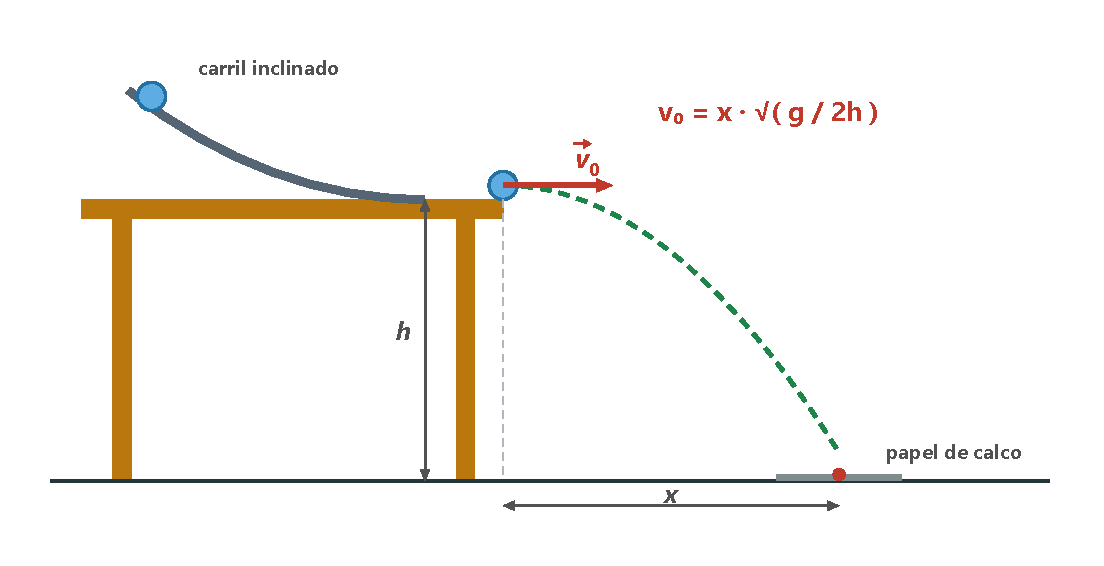
\includegraphics[width=0.7\textwidth]{images/UD9/mesa_rampa}
    \caption{La canica sale de la mesa con velocidad horizontal y cae describiendo media parábola.}
    \label{fig:ud9-mesa}
\end{figure}

\textbf{Procedimiento}
\begin{enumerate}[label=\numberballgreen]
    \item Coloca la rampa sobre la mesa de modo que la canica salga por el borde con velocidad horizontal. Mide la altura \(h\) de la
    mesa.
    \item Pega en el suelo una hoja de papel blanco con papel de calco encima, donde caiga la canica: cada impacto deja una marca.
    \item Suelta la canica siempre desde el mismo punto de la rampa, unas diez veces, y mide la distancia \(x\) desde la vertical del
    borde de la mesa hasta el centro de las marcas.
    \item Repite la experiencia soltándola desde otras alturas de la rampa.
\end{enumerate}

\begin{exercise}
    a) Demuestra que la velocidad con la que la canica sale de la mesa es \(v_0 = x\sqrt{\dfrac{g}{2h}}\). b) Con una mesa de
    \qty{80}{\cm} de altura, la canica cae a \qty{48}{\cm} del borde. Calcula el tiempo de caída y la velocidad de salida. c) ¿Qué
    ocurre con el alcance si la canica sale con el doble de velocidad? ¿Y con el tiempo de caída?
    \begin{solu}
        a) \textcolor{blue}{Tiempo de caída: \(h = \frac{1}{2}\,g\,t^2 \Rightarrow t = \sqrt{2h/g}\); avance horizontal: \(x = v_0\,t\).}
        Despejando, \(\textcolor{red}{v_0 = x/t = x\sqrt{g/(2h)}}\). b) \(t = \sqrt{\num{1.6}/\num{9.8}} = \textcolor{red}{\qty{0.404}{\s}}\);
        \(v_0 = \dfrac{\num{0.48}}{\num{0.404}} = \textcolor{red}{\qty{1.19}{\m\per\s}}\). c) \textcolor{red}{El alcance se duplica,
        pero el tiempo de caída no cambia}: solo depende de la altura.
    \end{solu}
\end{exercise}

%========================================================================================
\section{Situación de aprendizaje: velocidad, seguridad y clima (ODS 13)}\label{sec:ud9-ods}
%========================================================================================

Los vehículos de combustión son una de las principales fuentes de los gases de efecto invernadero y de la contaminación del aire en
las ciudades. Por eso muchas ciudades han creado \textbf{zonas de bajas emisiones}, en las que solo pueden circular los vehículos con
ciertos \textbf{distintivos ambientales} de la DGT (0, ECO, C y B, según sus emisiones), y han reducido los límites de velocidad: la
mayoría de las calles urbanas de un solo carril por sentido están limitadas a \qty{30}{\km\per\hour} desde 2021, y hay calles
escolares limitadas a \qty{20}{\km\per\hour}. El \textbf{ODS 13} (acción por el clima) pide adoptar medidas urgentes para combatir el
cambio climático y sus efectos.

Reducir la velocidad tiene además otra ventaja que podemos calcular con la cinemática: la \textbf{distancia de detención}. Cuando un
conductor ve un peligro, tarda un tiempo en reaccionar (alrededor de \qty{1}{\s}) durante el que el coche sigue a la misma velocidad
(MRU), y después frena (MRUA).

\begin{marker}
    \textbf{Reto:} preparad por grupos un informe sobre las medidas de movilidad y clima de vuestra localidad, con cálculos que
    muestren por qué se limita la velocidad en las ciudades.
\end{marker}

\begin{enumerate}[label=\numberballred]
    \item \textbf{Investigad.} ¿Qué medidas ha tomado vuestro ayuntamiento para reducir la contaminación del tráfico? ¿Qué significa
    cada distintivo ambiental y dónde se exige?
    \item \textbf{Calculad} la distancia de detención de un coche a 20, 30, 50 y \qty{70}{\km\per\hour}, con un tiempo de reacción de
    \qty{1}{\s} y una aceleración de frenado de \qty{-7}{\m\per\s\squared}. Representadla frente a la velocidad.
    \item \textbf{Comparad} los coches de combustión, los eléctricos de batería y los de pila de combustible de hidrógeno: cuatro
    semejanzas y cuatro diferencias (energía que usan, emisiones, autonomía, precio, infraestructura de recarga).
    \item \textbf{Comunicad} vuestras conclusiones con cinco acciones por el clima relacionadas con el transporte que podáis llevar a
    cabo vosotros mismos.
\end{enumerate}

\begin{exercise}
    Resuelve el apartado 2 de la situación de aprendizaje. ¿Por cuánto se multiplica la distancia de detención al pasar de 30 a
    \qty{50}{\km\per\hour}?
    \begin{solu}
        \textcolor{blue}{\(d = v\,t_r + \dfrac{v^2}{2 \cdot 7}\), con \(v\) en m/s.} \textcolor{red}{A \qty{20}{\km\per\hour}
        (\qty{5.56}{\m\per\s}): \(\num{5.6} + \num{2.2} = \qty{7.8}{\m}\); a 30 (\num{8.33}): \(\num{8.3} + \num{5.0} =
        \qty{13.3}{\m}\); a 50 (\num{13.9}): \(\num{13.9} + \num{13.8} = \qty{27.7}{\m}\); a 70 (\num{19.4}): \(\num{19.4} +
        \num{27.0} = \qty{46.4}{\m}\).} La distancia \textcolor{red}{se multiplica por más de 2} (\(\num{27.7}/\num{13.3} =
        \num{2.1}\)): la parte de frenado crece con el cuadrado de la velocidad.
    \end{solu}
\end{exercise}
